\mainmatter

\chapter{Introduzione}
 
Il basso peso alla nascita \`e una delle maggiori cause di morbilit\`a e mortalit\`a
nel periodo neonatale e nell'infanzia in tutto il mondo.
Inoltre osservazioni epidemiologiche hanno evidenziato un aumentato rischio di 
alterazioni metaboliche e malattie cardiovascolari nei soggetti nati piccoli 
per l'et\`a gestazionale (SGA)\cite{consensus}.

Infine il 10-15\% dei bambini SGA è destinato a non raggiungere la statura normale\cite{sga}.

\section{Definizione di SGA}

In base ai dati antropometrici rilevati alla nascita, i neonati vengono classificati come:
\begin{itemize}
\item piccoli per l'epoca gestazionale (SGA - small for gestational age) quando presentano peso e/o lunghezza inferiori al 3°
   percentile o alle -2SD rispetto alle curve di normalità per sesso relative ad una popolazione di appartenenza ;
\item adeguati per l'epoca gestazionale (AGA - adeguate for gestational age) quando presentano peso e/o lunghezza compresi
   fra il 3° e il 90° percentile;
\item grandi per l'epoca gestazionale (LGA - large for gestational age) quando presentano peso e/o lunghezza superiori
   al 90° percentile\cite{sga-1}.
\end{itemize}

Occorre notare che la definizione SGA non considera alcuni fattori di fondo che modificano la crescita, come la taglia fisica della madre,
l'etnia e la gemellarit\`a\cite{consensus}.
L'acronimo SGA è spesso erroneamente considerato sinonimo di IUGR (Intrauterine Growth Retardation), pur non essendo i due termini
equivalenti\cite{sga}: la definizione di IUGR è primariamente di tipo ostetrico, basata su due misurazioni ecografiche che evidenzino la ridotta crescita fetale\cite{consensus}.
Un neonato che ha presentato un ritardo di crescita intrauterino non necessariamente pu\`o essere classificato come uno SGA,viceversa un
neonato SGA pu\`o essere definito IUGR. Infatti un feto n\`e  che presenta un rallentamento intrauterino della crescita può collocarsi dal punto di vista 
auxologico alla nascita anche sopra le -2SD\cite{sga}.

\section{Prevalenza dei nati SGA}

Circa il 3-10\% dei nati in tutto il mondo sono piccoli per l'età gestazionale, 
ma questo dato è decisamente sottostimato: nei Paesi poveri in via di sviluppo 
e del terzo mondo i neonati spesso non vengono pesati e misurati\cite{sga-1}.
In Piemonte nascono ogni anno 800 bambini SGA. Di questi, 80 non presentano crescita di recupero: si tratta di un numero 8 volte superiore all'incidenza di deficit di GH (fonte ISTAT 2005).  


\section{Cause}

%Le cause del ritardo di crescita intrauterino si dividono in:
%\begin{itemize}
%\item cause intrinseche o fetali,
%\item cause estrinseche o materno -- placentari.
%\end{itemize}

Le cause del ritardo di crescita intrauterino si dividono in
fetali (dette intrinseche) e materno -- placentari (estrinseche).


Tra le più frequenti cause intrinseche vi sono le infezioni, che possono determinare una sofferenza
fetale con una riduzione del normale accrescimento. 
Inoltre le anomalie genetiche (ad esempio S. di Silver Russell), le sindromi cromosomiche (come S. di Turner, S. di Cornelia de Lange), le malformazioni congenite e la gemellarità rappresentano
ulteriori fattori che agendo direttamente sul feto ne ritardano frequentemente la crescita.


Le cause estrinseche si presentano tipicamente nelle fasi tardive della gravidanza
e comportano un ridotto apporto di nutrienti e/o di ossigeno solitamente dovuti alla presenza di 
gestosi, di insufficienza placentare oppure ad un'inadeguata alimentazione materna.


\`E infatti emerso che le donne con figli AGA presentavano una dieta più ricca in carboidrati,
frutta, ferro ed acido folico rispetto a donne con figli SGA. Si è visto che è soprattutto la
supplementazione di acido folico già al momento del concepimento a ridurre il rischio di 
avere figli piccoli per l'età gestazionale, nonché il rischio di mielomeningocele nel nascituro.\cite{sga-26}


Tra le cause estrinseche vanno inclusi anche i farmaci come i chemioterapici, gli anticomiziali
e gli agenti chimici che vengono in contatto col feto tramite la madre.
Bisogna considerare anche il tipo di attivit\`a lavorativa, con l'ammontare delle ore
che vi vengono dedicate durante la gestazione: \`e noto che il lavoro pesante, 
richiedente un impegno fisico importante o uno sforzo prolungato, soprattutto se nell'ultimo trimestre,
può determinare parto pretermine, eclampsia, rottura prematura delle membrane e nascita di 
neonati IUGR e/o SGA\cite{sga-14}.


Alcuni lavori riportano un rischio aumentato di presentare gravidanze complicate
in donne con celiachia non diagnosticata; tale constatazione si basa su immunologia e 
su background nutrizionale, poich\'e l'infiammazione del piccolo intestino causa uno
scarso assorbimento di sostanze nutritive e di conseguenza non concede al feto un apporto alimentare adeguato,
determinandone il ridotto accrescimento\cite{sga-15}.


La gravidanza \`e influenzata negativamente dal fumo di sigaretta in tutta la sua evoluzione.
Le donne fumatrici in gravidanza sono il 23,7\% delle gestanti (sondaggio ISTAT 2001).
Il Centro Internazionale di Consultazione sul fumo ha concluso che il tabagismo durante la gestazione
\`e la maggiore causa di basso peso alla nascita\cite{sga-18}.


Si \`e verificata altres\`i l'importanza del fumo passivo. I metaboliti del tabacco agiscono creando
una situazione di ipossia fetale soprattutto tramite due meccanismi: la formazione di carbossi -- emoglobina, 
per legami di emoglobina e monossido di carbonio; l'aumento della secrezione di catecolamine plasmatiche
dalla midollare del surrene con conseguente vasocostrizione dell'arteria uterina e di quella ombelicale
con riduzione dell'afflusso ematico al feto\cite{sga-20}.
Anche l'abuso di sostanze stupefacenti e/o di alcolici è coinvolto nei meccanismi sopracitati\cite{sga-24}\cite{sga-25}.


Va inoltre notato che sussiste una maggiore probabilità di avere figli piccoli per l'et\`a gestazionale
da parte di quelle donne il cui peso alla nascita fosse inferiore al terzo centile.
Ciò suggerisce un'ereditarietà delle dimensioni alla nascita trasmessa per via materna. Sebbene
i geni con imprinting non rappresentino oltre lo 0,5\% dell'intero genoma, essi svolgono
però un ruolo importante nel regolare lo sviluppo fetoplacentare, controllando l'accrescimento, la 
morfologia e la capacità di scambio di nutrienti tra la placenta e il feto.
In particolare il gene IGF-II sembra essere fortemente coinvolto nella regolazione dello sviluppo
fetoplacentare. L'importanza dell'imprinting genico è dimostrata dall'effetto della disomia uniparentale
nell'uomo e nei roditori: l'accrescimento è stimolato dalle disomie paterne, mentre \`e inibito da quelle materne.\cite{fowden2006imprinted}


Infine occorre considerare che esiste un enorme divario tra paesi in via di sviluppo e industrializzati.


Nei paesi in via di sviluppo le principali cause di dismaturità includono il fumo, l'inadeguato stato di 
nutrizione materna, la giovane età della gravida nonché le infestazioni del Plasmodium della malaria a 
livello placentare.


Nei paesi industrializzati la nascità di bambini piccoli per l'età gestazionale
è spesso legata alla gemellarità (favorita da pratiche di fecondazione assistita
e dall'elevata età materna) oppure alla dieta restrittiva e rigida della gestante.


L'insufficienza utero-placentare di grado lieve-moderato che si manifesta dopo la 
ventiseiesima settimana di gestazione compromette soprattutto la biometria addominale: 
in condizioni di scarso afflusso sanguigno viene privilegiato lo sviluppo degli 
organi nobili (cervello, cuore, surrene) a scapito della massa epatica,che va incontro ad ipotrofia cellulare. 
Qusta situazone porta ad un ritardo di crescita disarmonico (SGA asimmetrico).


Le cause intinseche (in particolare le malattie genetiche e le infezioni contratte 
nei primi mesi di gravidanza) o l'insufficienza utero-placentare severa ad esordio 
precoce hanno un impatto pi\'u importante sullo sviluppo fetale, comportando un'ipocellularità con 
riduzione sia della circonferenza addominale, che della lunghezza degli arti e 
della circonferenza cranica. In tal caso si parla di SGA simmetrico, altrimenti detto "`low profile"' o armonico.


La distinzione fra SGA asimmetrici e simmetrici \`e importante: studi osservazionali 
hanno dimostrato che i bambini con deficit prevalentemente ponderale alla nascita 
(SGA asimmetrici) presentano una migliore prognosi staturale rispetto agli SGA simmetrici.\cite{sga-10}

\begin{table}[h]\centering
\begin{tabular}{cll}
\toprule
			& \multicolumn{1}{c}{Paesi sviluppati}			& \multicolumn{1}{c}{Paesi in via di sviluppo} \\
\midrule
Intrinseche & Gemellarit\`a 			& Infezioni			\\\midrule
\multirow{4}{*}{Estrinseche} & Fumo						& Fumo/povertà		\\\cmidrule(l){2-3}
			& Fecondazione assistita	& Inadeguata nutrizione materna	\\\cmidrule(l){2-3}
			& Avanzata età materna (primigravida) &	Giovane età materna \\\cmidrule(l){2-3}
			& Disfunzioni placentari	& Eccessivo carico di lavoro	\\\bottomrule
\end{tabular}
\label{tab-cause}
\caption{Cause e conseguenze di essere nato SGA in correlazione al paese di origine.}
\end{table}

  

\section{Complicanze}


Per spiegare le complicanze a cui tendono ad andare incontro i soggetti nati SGA è stato proposto il modello del fenotipo risparmiatore (\textit{Thrifty phenotype}).
Secondo questa ipotesi, la malnutrizione intrauterina sarebbe il fattore scatenante
per innescare nel feto una serie di meccanismi di adattamento indispensabili per 
la sua sopravvivenza a breve termine, ma che comportano delle modificazioni permanenti
del metabolismo energetico.
Tali meccanismi di adattamento avvengono per favorire lo sviluppo dei tessuti 
nobili come quello nervoso, cardiaco e renale, a scapito di altri tessuti.

In particolare sembrerebbe instaurarsi una riduzione della sensibilità all'insulina
a livello periferico condizionante il calo della glicogenesi e della lipogenesi
con raggiungimento di livelli plasmatici ottimali di glucosio e acidi grassi liberi
indispensabili per un corretto sviluppo del sistema nervoso e degli organi splacnici.\cite{sga-51}



\`E possibile distinguere conseguenze a breve e lungo termine che tale risposta
adattativa produce nei soggetti coinvolti.

Tra le ripercussioni immediate la più importante riguarda lo scarso accrescimento
staturo-ponderale presente sia a livello intrauterino che post nascita. Inoltre 
il nato piccolo per l'età gestazionale tende ad accumulare grasso in depositi a livello
viscerale a discapito di una corretta formazione di massa magra. L'accelerazione e 
l'attivazione anticipate di processi fisiologici costituiscono un ulteriore tipo di 
effetto a breve termine: spesso si assiste alla ricerca di un tempo gestazionale
rapido (prematurità) al fine di ridurre la permanenza in un ambiente stressante
e non ottimale per l'accrescimento.\cite{sga-53}

Le conseguenze a lungo termine comprendono un ridotto sviluppo cognitivo, disturbi emozionali e di comportamento nei 
soggetti che non presentano una normalizzazione nella circonferenza cranica;soprattutto nelle bambine, pubertà 
anticipata ed a rapida progressione  che determina una perdita di 
statura nell'età adulta; malattie della sfera glicometabolica (ridotta sensibilità insulinica, diabete mellito,
ipertensione arteriosa, sovrappeso e obesità).\cite{sga-32}


\section{Crescita nei bambini SGA}

I soggetti nati SGA tendono, come popolazione, a essere degli adulti più piccoli
rispetto ai nati con dimensioni appropriate all'età gestazionale. In uno studio
a lungo termine condotto su 213 soggetti SGA e 272 con peso alla nascita normale, il 
13,6\% degli individui nati SGA presentava una statura inferiore a -2 DS all'età di
20-21 anni, contro solo l'1.8\% del gruppo di controllo.\cite{leger1997reduced}

La statura media degli adulti nati SGA è di circa 1 DS al di sotto della altezza 
media della popolazione. Tipicamente il bambino SGA presenta, nei primi 6-12 mesi
di vita, una accellerata crescita lineare (\textit{catch up growth}) che nel 90\%
dei casi permette il raggiungimento di una statura superiore a -2 DS all'età di
2 anni\cite{karlberg1995growth}.
Si è ipotizzato che ciò avvenga mediante rallentamento della senescenza dei condrociti.\cite{gafni2001catch}
La crescita di recupero ha più successo quando avviene nella prima e seconda infanzia (entro i quattro anni di vita), poichè in quel periodo la velocità di crescita staturale è molto elevata. %citare Tanner,1994

\begin{figure}[!h]
  \begin{center}
      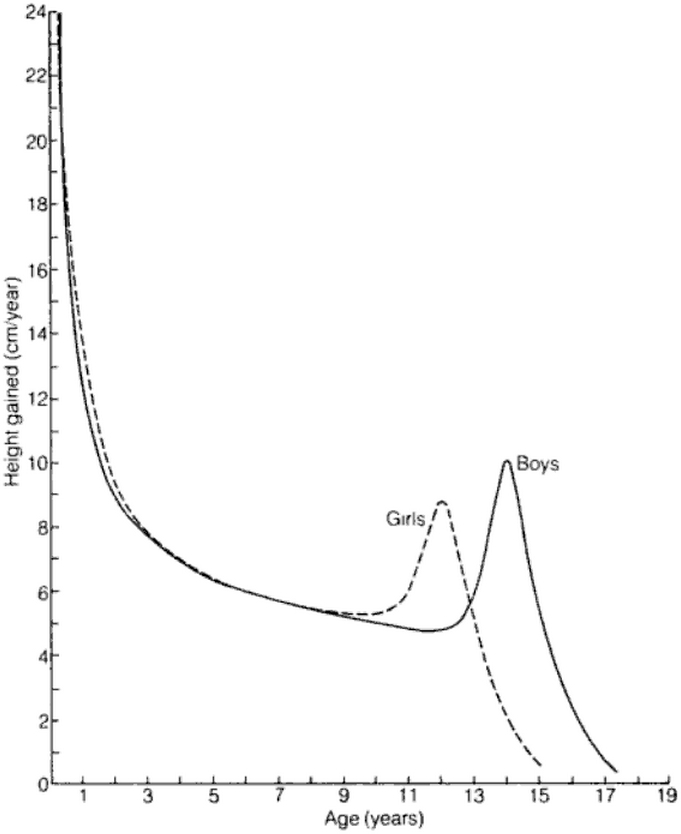
\includegraphics[scale=0.40]{grafici/curva-velocita} %\\
  \end{center}
  \caption{Curve delle velocità di crescita in altezza.}
  \label{fig:VelocitaCrescita}
\end{figure}

Circa il 10\% dei nati SGA non recupera e rimane definitivamente al di sotto delle -2 DS.
Il rischio relativo di bassa statura all'età di 18 anni, tra i bambini nati SGA
che non presentano un recupero sufficiente nei primi 2 anni di vita è 5,2 per quelli 
piccoli in peso e 7,1 per quelli piccoli in lunghezza.
La lunghezza alla nascita e la statura dei genitori sono importanti variabili predittive della statura da 
adulto: i bambini con lunghezza alla nascita minore sono a maggior rischio di bassa statura;
quelli con genitori alti hanno una maggiore probabilità di raggiungere
un'altezza normale da adulti.\cite{cianfarani2006hormonal}

Tuttavia è importante notare come questi parametri aiutino a quantificare un 
rischio relativo "generico" ma non permettano di identificare con precisione 
i bambini SGA destinati al recupero staturale.

Infatti la relazione tra l'eziologia del ritardo di crescita fetale e l'andamento della 
crescita postnatale non è chiaramente definita.
Né le concentrazioni circolanti di GH, IGF-I, proteina-3 legante l'IGF-I, n\'e l'indice
di massa corporea, sono infatti predittivi della successiva crescita.\cite{consensus}

La pubertà sovente anticipata e/o a rapida progressione è un'altra causa di bassa statura nei soggetti nati SGA. Infatti l'altezza finale dipende prevalentemente dalla velocità di crescita prepuberale nei maschi, nelle femmine anche dalla durata di crescita prepuberale; il guadagno in altezza che si ottiene durante lo scatto puberale è legato soprattutto alla durata dello scatto\cite{gasser1985human}.

